\documentclass[a4paper,12pt]{article}
\usepackage{graphicx}
\usepackage[UTF8]{ctex}
\usepackage{fontspec}
\usepackage{booktabs}
\usepackage{float}%浮动体
\usepackage{amsmath,amssymb}
\usepackage{fancyhdr}
%\usepackage{xcolor}
\usepackage{colortbl}
\usepackage{geometry}
\geometry{top=2cm,bottom=2cm,left=1cm,right=1cm}
\begin{document}
	\begin{figure}[H]
	\begin{center}
		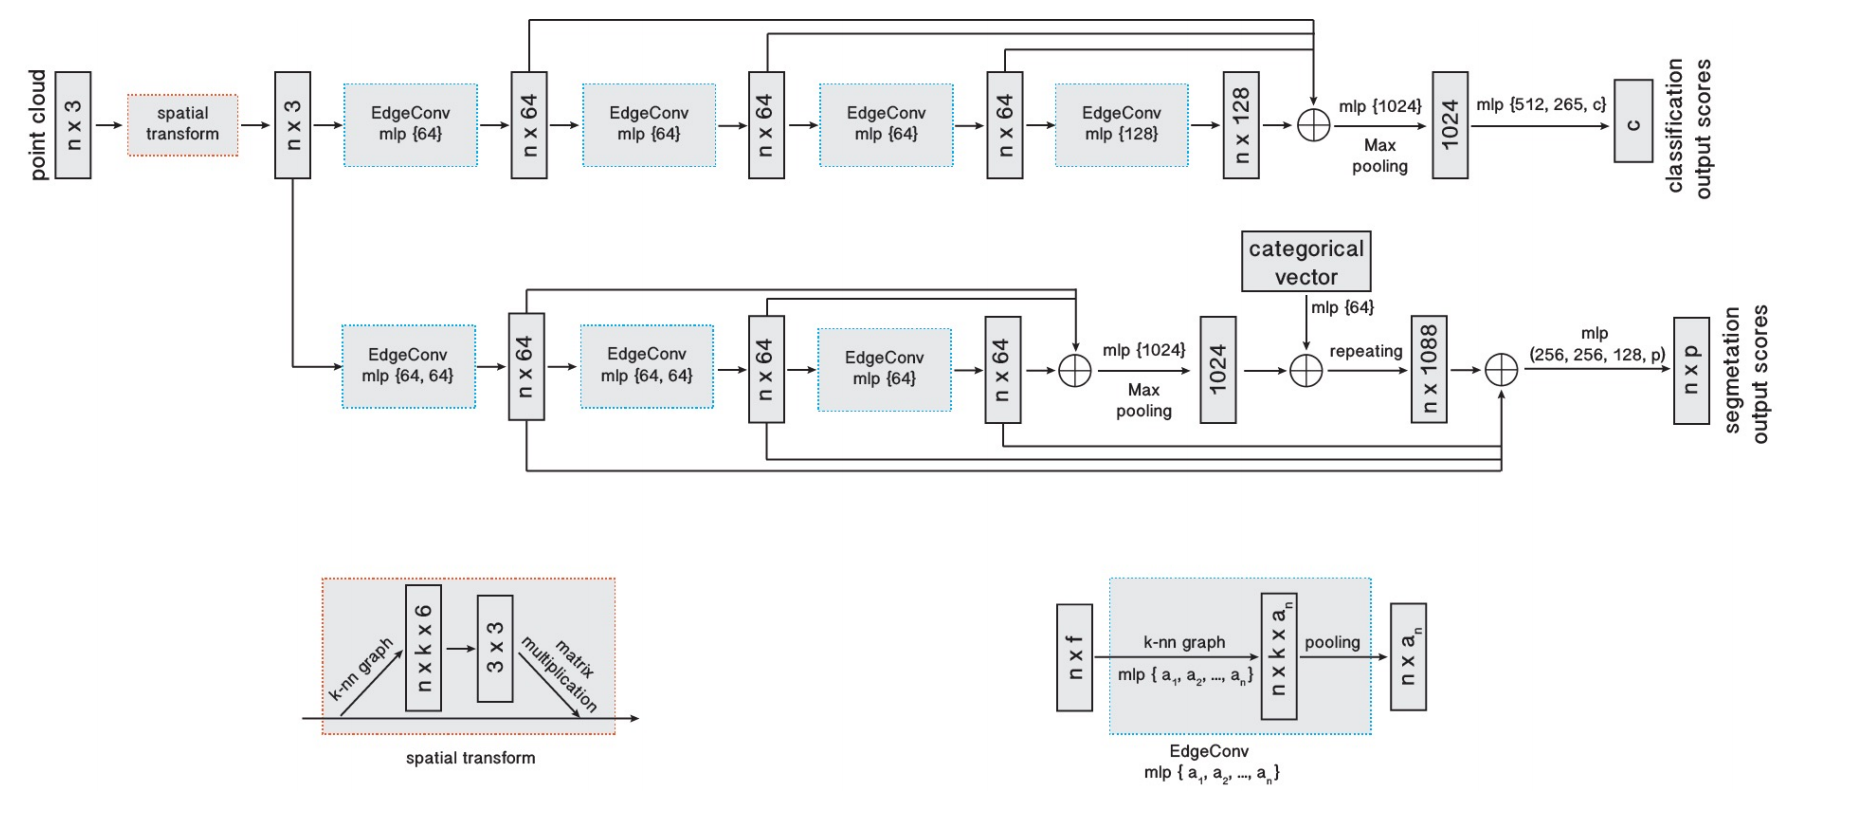
\includegraphics[width=0.9\textwidth]{img/DGCNN.png} 
		\caption{DGCNN}
	\end{center}
\end{figure}

\textbf{EdgeConv}:
\begin{itemize}
	\item 用KNN的方法选取K个点。来构成一张图。中心位置是$x_i$
	\item 然后将$x_i$的特征和$x_j - x_i$的特征叠加[$x_i$, $x_j-x_i$]
	\item 随后进行卷积,ReLU,和pooling操作。
\end{itemize}

$$
h_{\Theta}\left(\mathbf{x}_{i}, \mathbf{x}_{j}\right)=\bar{h}_{\Theta}\left(\mathbf{x}_{i}, \mathbf{x}_{j}-\mathbf{x}_{i}\right)
$$
$$
e_{i j m}^{\prime}=\operatorname{ReLU}\left(\boldsymbol{\theta}_{m} \cdot\left(\mathbf{x}_{j}-\mathbf{x}_{i}\right)+\boldsymbol{\phi}_{m} \cdot \mathbf{x}_{i}\right)
$$
$$
x_{i m}^{\prime}=\max _{j:(i, j) \in \mathcal{E}} e_{i j m}^{\prime}
$$
$$\Theta=\left(\theta_{1}, \ldots, \theta_{M}, \phi_{1}, \ldots, \phi_{M}\right)$$


\paragraph{分类任务}
如图1
\paragraph{语义分割} 如图1

\end{document}